\chapter{Grundlagen}
\label{chap:basics}
\todo[size=\small, inline, color=yellow]{Grundlagen $\rightarrow$ Spellcheck!}
\todo[size=\small, inline]{Evtl. besseren Namen für Kapitel "`Grundlagen"' finden $\rightarrow$ Grundlegende Algorithmen/Techniken?!}%
\textbf{Hier kommt nur rein was ICH mache!}\\
An dieser Stelle soll zunächst ein Überblick über die in der vorliegenden Arbeit verwendeten Techniken gegeben werden. Diese beinhalten unter anderem Algorithmen der Computergrafik, welche Datenstrukturen benutzt werden und wie die Speicherverwaltung organisiert ist.

\section{Datenstrukturen}
\label{sec:basics:datenstrukturen}
\textbf{Wofür und warum?!}\\
3D-Modelle aus Computer Aided Design - Anwendungen (CAD) werden üblicherweise nach ihrer Funktion gruppiert. Das mag beim Entwurf solcher Systeme auch praktisch sein, bei der Visualisierung kann dies jedoch zu Problemen führen. Bei CAD-Modellen in Größenordnung der Boeing 777\footnote{\todo[size=\small, inline]{Boeing Herkunftshinweis verschieben an die erste Stelle wo es erwähnt wird.}%
Das 3D-Modell der Boeing 777 wurde freundlicherweise zur Verfügung gestellt von The Boeing Company, Seattle, WA, USA.} (ca. 350 Millionen Dreiecke) ist es wichtig, dass diese in eine geeignete räumliche Unterteilung überführt werden. Da ein Out-Of-Core-Renderer entwickelt wurde, findet ein ständiges Laden und Verwerfen von Teilmodellen statt. Je länger ein Renderer benötigt um herauszufinden, welche Teile des Modells er verwerfen kann und welche er als erstes anfordern sollte, desto länger braucht er auch um ein Bild zu erstellen. In dieser Arbeit wurde als hierarchische räumliche Unterteilung ein Randomized Sampletree (\ref{sec:basics:sampletree}) und zum Vergleich ein Loose Octree gewählt.

\subsection{Loose Octree}
\label{sec:basics:octree}
Um einen Octree\footnote{\cite{RTR3}, Seiten 647 ff.} zu Erzeugen wird die gesamte Szene in eine minimale Boundingbox eingeschlossen. Rekursiv wird diese Box entlang der drei räumlichen Achsen in der Mitte geteilt, woraus sich jeweils acht gleich-große Boundingboxen ergeben. Dieser Vorgang wird so lange wiederholt bis ein Haltekriterium erfüllt ist. Im Falle der Boeing wurde festgelegt, dass höchstens 5.000 Dreiecke in einer Box liegen dürfen und die maximale Tiefe des Baums wurde auf 14 beschränkt. Erfüllt ein Octree-Knoten eines dieser Kriterien, wird nicht weiter untereilt. Dementsprechend gibt es keine leeren Blatt-Knoten im Octree. In Abbildung \ref{fig:basics:octree} ist ein Octree zu sehen.\\
\begin{figure}
 \centering
  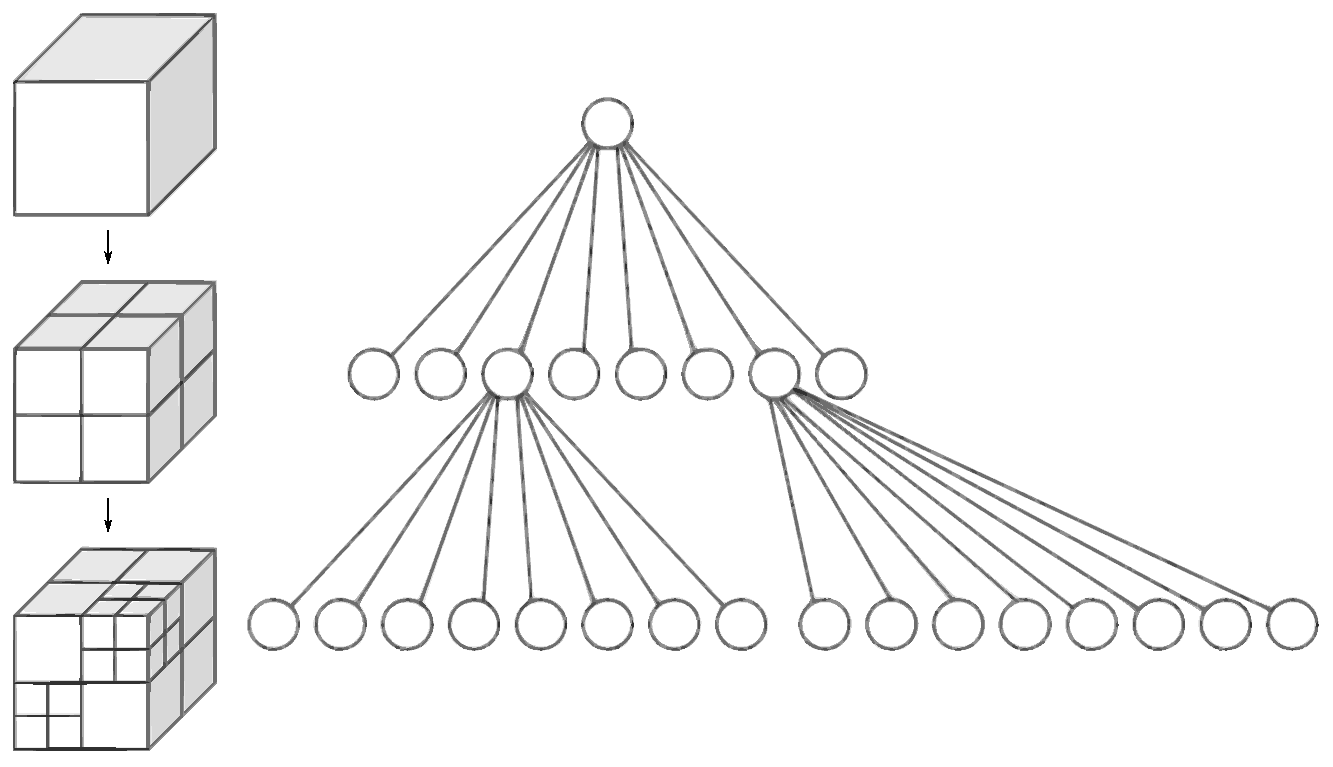
\includegraphics[scale=0.5]{images/octree.pdf}
 % octree.pdf: 640x368 pixel, 72dpi, 22.58x12.98 cm, bb=0 0 640 368
  \caption{Ein Octree der Tiefe 2. \textit{links: die räumliche Darstellung, rechts: die Baumdarstellung. Quelle: \htmladdnormallink{http://de.wikipedia.org/wiki/Octree}{http://de.wikipedia.org/wiki/Octree}}}
 \label{fig:basics:octree}
\end{figure}
In dieser Arbeit wurde jedoch eine spezielle Form des Octrees verwendet: der Loose Octree. Dieser erweitert den Octree um eine weitere Box pro Knoten: die sogenannte Loosebox. Sie teilt sich ihr Zentrum mit der Octree-Boundingbox, besitzt aber doppelte Kantenlängen. Wird nun festgestellt, dass in einem Knoten mehr als 5.000 Dreiecke liegen, wird die größe der einzelnen Dreiecke anhand der Loosebox geprüft. Liegt ein Dreieck vollständig in der Loosebox mit seinem Zentrum in der eigentlichen Boundingbox des Knotens, kann es weiter nach unten gereicht werden. Ist dies nicht der Fall, ist das Dreieck zu groß für den aktuellen Knoten und wird an den Vaterknoten gegeben (Abbildung \ref{fig:basics:looseoctree}).\\
Dies hat den Vorteil, dass große Dreiecke relativ weit oben im Baum zu liegen kommen und Kleinere entsprechend tief. Je größer ein Dreieck ist, desto größer ist auch die Wahrscheinlichkeit, dass das Dreieck sichtbar ist und somit gezeichnet werden muss. Bewegt man sich durch ein Modell, ist der Wurzelknoten, oder Szenen-Boundingbox, praktisch immer sichtbar, was bedeutet, dass die zur Wurzel gehörige Geometrie gezeichnet werden muss.
\begin{figure}
 \centering
  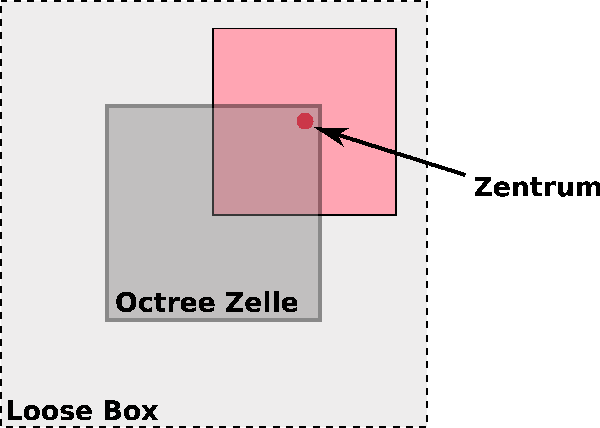
\includegraphics[scale=0.8]{images/looseoctree2.pdf}
  \caption{Ein Loose Octree in einer 2D-Darstellung. \textit{Das Zentrum des Objekts (rosa) befindet sich innerhalb der Octree Zelle, das gesamte Objekt befindet sich innerhalb der Loose Box. Quelle: nach \htmladdnormallink{http://anteru.net/2008/11/14/315/}{http://anteru.net/2008/11/14/315/}}}
 \label{fig:basics:looseoctree}
\end{figure}

\subsection{Randomized Sampletree}
\label{sec:basics:sampletree}
Als spezielle Ausprägung eines Loose Octrees gibt es den Randomized Sampletree \cite{klein}. Dieser unterschiedet sich von einem Octree darin, dass zufällig einzelne Dreiecke aus tieferen Knoten in höhere Knoten verschoben  wurden. Beim rendern der Szene wird in jedem Frame der Baum traversiert, um ein Frustum-Culling durchzuführen (siehe auch \ref{sec:basics:algos}). Ab einer bestimmten Tiefe im Baum wird die Traversion abgebrochen, um die Komplexität der Darstellung zu reduzieren. Dadurch kommt es allerdings zu Darstellungsfehlern, da nicht alle sichtbare Geometrie gerendert wird. An dieser Stelle schafft ein Randomized Sampletree abhilfe. Dadurch dass zufällige kleinere Dreiecke in höherliegenden Knoten gespeichert sind, werden diese auch gerendert. Ist die Flächensumme alle Dreiecke in einem Knoten des Sampletrees nicht größer als ein Pixel, wird die Traversion abgebrochen. Klein, Krokowski und Fischer \cite{klein} haben gezeigt, dass diese Geometrie-Approximation von weit entfernten Objekten durch zufällige Dreiecke eine hinreichend korrekte Darstellung liefert. Dieses Verfahren wurde für komplexe geometrische Umgebungen entwickelt, weshalb es in dieser Arbeit verwendet wurde.
\begin{figure}
 \centering
  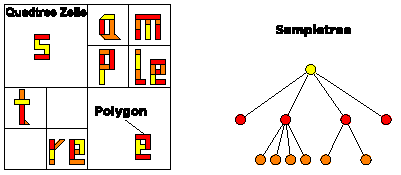
\includegraphics[scale=1.7]{images/sampletree2.pdf}
  \caption{Ein Sampletree in einer 2D-Darstellung. \textit{links: Eine Aufteilung von Polygonen in verschiedene Quadtree Zellen. rechts: Die Baumdarstellung des Sampletrees. Die farbigen Knoten geben an welche Polygonteile der linken Seite in welchen Knoten gespeichert wurden. Quelle: nach \cite{klein}}}
 \label{fig:basics:sampletree}
\end{figure}

\section{Computergrafik}
\label{sec:basics:computergrafik}
\todo[size=\small, inline]{Pipeline-Stall/Flush bei Farbsetzung muss nochmal gegengeprüft werden!}
Da Arbeitsspeicher in der Regel größer ist als der Speicher einer Grafikkarte, werden nicht alle geometrischen Objeke auf der Grafikkarte belassen. Wenn angeforderte Objekte bei einem Renderer eintreffen, werden die zunächst gar nicht an die Grafikkarte geschickt. Erst nach weiteren Tests, ob das Objekt immer noch sichtbar ist, findet der transfer zur GPU statt. Dort verbleiben sie dann, bis sie irgendwann aus platz- oder sichbarkeitsgründen verdrängt werden (siehe auch \ref{sec:basics:caching}). Um dies möglichst effizient umsetzen zu können werden Vertexbuffer Objects  (VBOs) genutzt. Die Idee ist dabei, dass Modelldaten, bestehend aus Vertices und Vertex-Normalen, in einem zusammenhängenden Speicherblock abgelegt werden. Ein Vertex besteht aus einer $xyz$-Koordinate und einer Vertex-Normalen. Der Zugriff auf Dreiecke erfolgt dann mittels einer Index-Liste, bei der immer drei Indices ein Dreieck ergeben. Alle Dreiecke eines Octree-Knotens wurden zu einem Vertexbuffer-Objekt zusammen gefasst (siehe \ref{sec:basics:octree}), da Geometrie innerhalb eines Knotens nicht weiter unterteilt wird. In Form von VBOs kann recht einfach entsprechender Platz im Grafik-RAM reserviert und die Daten in den Speicher geladen werden.\\
Im Gegensatz dazu verbleiben bei Vertex-Arrays alle Daten im Arbeitsspeicher des Rechners und werden für jeden Zeichenaufruf zur Grafikkarte übertragen. Vertex-Arrays bieten sich an, wenn Objekte nur einmal gezeichnet und dann verworfen werden. Von daher kommen sie nur auf den Datenknoten (siehe \ref{sec:impl:netzwerkarchitektur}) zum Einsatz, da diese ein getestetes Objekt nur in ihren Tiefenbuffer rendern und dann wieder verwerfen. Bei VBOs wäre der Overhead der Datenübertragung und der anschließenden Deallokation zu groß für eine einmalige Verwendung.
\begin{figure}
  \centering
  %%%%%%%%%%%%%%%%%%%%%%%%%%%%%%%%%%%%%%%%%%%%%%%%%%%%%%%%%
% 1D-Farbtextur mit Beschreibung und Labels
%%%%%%%%%%%%%%%%%%%%%%%%%%%%%%%%%%%%%%%%%%%%%%%%%%%%%%%%%


\begin{tikzpicture}
  \tikzset{ 
    every pin/.style={fill=yellow!50!white,rectangle,rounded corners=3pt,font=\small}, 
    small dot/.style={fill=black,circle,scale=0.3} } 
  \begin{axis}[
    x=13cm, y=1.0cm, 
    clip=false,
    ytick=\empty,
    xtick={0,0.03125,0.0625,0.09375,0.125,0.15625,0.1875,0.21875,0.25,0.28125,0.3125,
      0.34375,0.375,0.40625,0.4375,0.46875,0.5,0.53125,0.5625,0.59375,0.625,
      0.65625,0.6875,0.71875,0.75,0.78125,0.8125,0.84375,0.875,0.90625,0.9375,
      0.96875,1},
    xticklabels={$0$,$\frac{1}{n}$,$\frac{2}{n}$,$\frac{3}{n}$,$\frac{4}{n}$,$\frac{5}{n}$,$\frac{6}{n}$,$\frac{7}{n}$,$\frac{8}{n}$,$\frac{9}{n}$,$\frac{10}{n}$,
      $\frac{11}{n}$,$\frac{12}{n}$,$\frac{13}{n}$,$\frac{14}{n}$,$\frac{15}{n}$,$\frac{16}{n}$,$\frac{17}{n}$,$\frac{18}{n}$,$\frac{19}{n}$,$\frac{20}{n}$,
      $\frac{21}{n}$,$\frac{22}{n}$,$\frac{23}{n}$,$\frac{24}{n}$,$\frac{25}{n}$,$\frac{26}{n}$,$\frac{27}{n}$,$\frac{28}{n}$,$\frac{29}{n}$,$\frac{30}{n}$,
      $\frac{31}{n}$,$\frac{32}{n}$},
       %tickpos=right,
    major tick length={0.07cm},
    xtick align=outside,
    xtick pos=left,
    tick style={very thin, black},
    tick label style={
    font=\tiny},
    %major x tick num=5,
    %hide y axis,
    enlargelimits=false,
    axis on top] 
    \addplot graphics [xmin=0,xmax=1,ymin=0,ymax=1, 
      % trim=left bottom right top 
      includegraphics={trim=0 9 0 8,clip}
      ] 
      {images/colors.pdf}; 

\node[small dot,pin=-90:{$\frac{1}{2n}$}] at (axis description cs:0.017625,0) {}; 
%\node[small dot,pin=-45:{$\frac{1}{n}$}] at (axis description cs: 0.03325,0) {}; 

  \end{axis} 
\end{tikzpicture}

  \caption{1D-Farbtextur. $n=$Anzahl Farben. Um mittig auf den Texel der Farbe $i$ zuzugreifen, errechnet sich die Texturkoordinate durch $\frac{i}{n}-\frac{1}{2n}$. }
  \label{fig:basics:1dtexture}
\end{figure}

Das Modell der Boeing 777 besitzt auch Farbinformationen. Da bei CAD-Modellen Farben oft einen Hinweis auf den Produktionsort geben, ist die Anzahl der Farben beschränkt. Natürlich könnte man jedem Vertex eine Farbe zuordnen. Dies hätte jedoch zur Folge dass bei jedem Vertex die Farbe neu gesetzt werden muss, unabhängig davon, ob diese Farbe bereits gesetzt ist. Das würde jedesmal die Grafik-Pipeline unterbrechen und es wäre mit Geschwindigkeitseinbußen zu rechen. Deshalb wurden die Farben der Boeing, 32 an der Zahl, in einer 1D-Textur kodiert und die Texturkoordinate wurde als vierte Komponente an den Vertex gehängt. Wird nun ein Vertex gezeichnet, ersetzt der Vertex-Shader die harmonische vierte Komponente eines Vertices wieder durch $1.0$ und gibt die Textur-Koordinate an den Fragment-Shader weiter. Letzterer muss ohnehin eine Farbe schreiben, weshalb diese kurzerhand aus der Textur ausgelesen wird. Da die Anzahl der Farben bekannt ist ist, ergibt sich zur Berechnung der Texturkorrdinate der $i$-ten Farbe $\frac{i}{n}-\frac{1}{2n}$, wobei $n=$  Anzahl der Farben ist (Abbildung \ref{fig:basics:1dtexture}). Die Subtraktion der Hälfte eines Texels $\frac{1}{2n}$ ist Notwendig, da man sonst genau auf die Kante zwischen zwei Farben zugreift, was zu undefiniertem Farbverhalten in der Grafikkarte führt.

\section{Algorithmen}
\label{sec:basics:algos}
In dieser Arbeit wurden verschiedene Algorithmen benutzt, welche an dieser Stelle näher erklärt werden sollen.

\subsection{Culling}
\label{sec:basics:algos:culling}
Ein elementarer Mechanismus zur Beschleunigung des Rendervorgangs ist das Culling. Damit lassen sich Szenenteile entfernen, die nicht zum finalen Bild beitragen, bevor eine Berechnung stattfindet. "`Das schnellste Polygon das man rendern kann ist jenes, welches gar nicht erst die Grafik-Pipeline betritt."'\footnote{nach \cite{RTR3}, Seiten 660 ff.}. Je nach Beschaffenheit einer 3D-Szene gibt es unterschiedlich viele Teile in einer solchen Szene, die nicht sichtbar sind. Sei es, weil sie außerhalb des Kamerasichtfelds (View-Frustum) liegen oder weil sie verdeckt sind. In Abbildung \ref{fig:basics:culling} sind die verschiedenen Culling-Techniken zu sehen, die auch in der Implementierung der vorliegenden Arbeit verwendet wurden (siehe Kapitel \ref{chap:impl}).
Einige dieser Cullung-Verfahren sind mittlerweile in Hardware implementiert und können direkt durch die API ein- und ausgeschaltet werden. Alle Techniken können aber auch auf der CPU implementiert werden. Der optimale Culling-Algorithmus würde ausschließlich alle sichtbaren Primitiven an die Pipeline übermitteln. Das Erzeugen solcher Datenstrukturen ist theoretisch auch möglich, aber nicht praktikabel, da die worst-case Zeitkomplexität solcher Algorithmen $O(n^{9})$ beträgt\footnote{laut \cite{culling}}. Stattdessen wird versucht, die Menge der Polygone zu ermitteln, die potentiell sichtbar sind (Potentialle Visible Set). Ist in so einem Potentially Visible Set (PVS) die Menge aller sichtbaren Polygone vollständig enthalten, wird das Verfahren als \textit{konservativ} bezeichnet. Ist sie nicht vollständig enthalten, nennt man es \textit{approximativ}. Letztere Art kann zu Fehlern im finalen Bild führen.

\begin{figure}
  \centering
  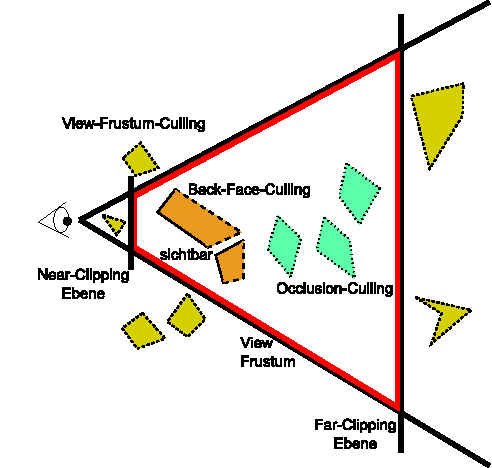
\includegraphics[scale=0.8]{images/culling.pdf}
  \caption{Verschiedene Culling-Techniken. Entfernte Geometrie ist durch gestrichelte Linien dargestellt. \textit{Quelle: nach \cite{culling}} }
  \label{fig:basics:culling}
\end{figure}
Beim Back-Face-Culling\footnote{\cite{RTR3}, Seiten 662 ff.} werden diejenigen Polygone entfernt, die vom Betrachter abgewandt sind. In Abbildung \ref{fig:basics:culling} würden bei den orangen Polygonen die vorderen Flächen gerendert, wobei die hinteren entfert würden (gestrichelte Linien). Dabei muss jede Fläche separat auf ihre Ausrichtung überprüft werden. In dieser Arbeit wird die von OpenGL angebotene Funktion für Back-Face-Culling verwendet.\\
View-Frustum-Culling entfernt Polygongruppen, die sich außerhalb des ViewFrustums befinden. In Abbildung \ref{fig:basics:culling} wären alle gelben Flächen außerhalb des Frustums (roter Bereich) davon betroffen. Alle Objekte, die sich vollständig oder partiell im Kamerabereich befinden, müssen gerendert werden. Da die Überprüfung von mehreren Millionen Dreiecken pro Frame zu teuer ist, werden lediglich die Boundingboxen von Objektgruppen getestet. Verwendet man zusätzliche räumliche Datenstrukturen, wie Octrees (siehe \ref{sec:basics:octree}), kann das Frustum-Culling hierarchisch durchgeführt werden. Dabei wird der Baum von der Wurzel bis zu dem Blättern durchlaufen. Liegt eine Boundingbox vollständig im Frustum, können alle Kindknoten ohne weitere Tests ebenfalls gezeichnet werden. Liegt eine Boundingbox vollständig außerhalb der Boundingbox, kann der Knoten samt aller Kindknoten entfernt werden, da diese ebenfalls außerhalb des Frustums liegen. Wird eine Box jedoch von einer Grenze des Frustums geschnitten, muss zum Einen die Geometrie im Knoten gerendert und die Kindknoten weiter getestet werden. Als weitere Möglichkeit zur Optimierung kann man sich diejenigen Grenzen speichern, die eine Box schneiden. Bei folgenden Tests der Kinder, müssen diese nur noch auf die gespeicherten Schnittflächen überprüft werden.\\
Soll vermieden werden, dass Objekte, die durch andere Polygongruppen verdeckt sind, gerendert werden, spricht man von Occlusion-Culling\footnote{\cite{RTR3}, Seiten 670 ff.}. Solche verdeckten Polygone würden in der Rendering-Pipeline transformiert, beleuchtet und anschließend gerastert, obwohl im fertigen Bild nicht davon sehen wäre. In Abbildung \ref{fig:basics:culling} sind die grünen Objekte vollständig verdeckt. Um mehrere Objekte auf ihre Sichtbarkeit zu überprüfen, wird gegen den Tiefenbuffer (Z-Buffer) getestet. Dazu muss schon ein Teil der Szene im Tiefenbuffer gerendert sein. Dabei ist die Zeichenreihenfolge wichtig. Gerendert wird in der Regel von vorne nach hinten in Abhängigkeit vom Standpunkt des Betrachters. Wird beispielweise bei der Boeing die Außenhülle als erstes gezeichnet, kann diese als Testgrundlage im Z-Buffer verwendet werden um das Innenleben, wird Letzteres wahrscheinlich nicht zu sehen sein. Dreht man die Reihenfolge um, müssen beide Teile gerendert werden. Entfernung von Objekten zur Kamera spielt ebenfalls eine Rolle. So kann eine Streichholzschachtel eine Golden Gate Bridge vollständig verdecken, wenn sich der Betrachter hinreichend dicht an der Streichholzschachtel befindet. Mittlerweile lässt sich Occlusion-Culling direkt auf der Grafik-Hardware durchführen. Dazu werden Occlusion-Queries verwendet, die nach dem Test ausgeben, wieviele Pixel der Objekte sichtbar sind. Dazu können vorher alle grafischen Effekte, wie Shader, Beleuchtung, usw, ausgeschaltet werden, um den Vorgang zu beschleunigen. Die Geschwindigkeit lässt sich noch verbessern, wenn statt der Originalgeometrie, nur Approximationen der Objekte gerendert werden. In dieser Arbeit wird Occlusion-Culling deshalb auf Boundingboxen durchgeführt. Dies kann jedoch zu falschen Testergebnissen führen. In Abbildung \ref{fig:basics:oculling} sind zwei verdeckte Objekte zu sehen. Beide befinden sich in der gleichen Boundingbox. Diese Box ist jedoch sichtbar und beide Objekte werden gerendert.

\todo[size=\small, inline]{Subsection-Titel ändern! Evtl. auch vorziehen bevor subsection Culling}
\subsection{Verschiedenes}
Das $c$-Collision Protokoll wird in Kapitel \ref{chap:relwork} genauer beschrieben. In dieser Arbeit wird es verwendet, um Datenanfragen möglichst gleichmäßig im Netzwerk zu verteilen. Jedes VBO (siehe \ref{sec:basics:computergrafik}) wird zufällig und redundant im Netzwerk verteilt. Alle Anfragen von allen Renderern werden jeden Frame gesammelt. Anschließend werden diese Anfragen zu Paketen gebündelt, die ebensoviele Anfragen enthalten wie es Datenknoten im Netzwerk gibt. Das $c$-Collision Protkoll wird immer auf einem Anfragenpaket ausgeführt. Begonnen wird  mit $c = 2$. Sollte in einer Runde kein weiterer Auftrag vergeben werden, obwohl noch offene Auftrage vorhanden sind, wird das $c$ erhöht. Dies wird so lange wiederholt, bis alle Aufträge vergeben sind.
\todo[size=\small, inline, color=magenta]{Kapitel: Algorithmen}

Da im Rahmen dieser Arbeit ein Sort-First-Renderer (siehe auch Kapitel \ref{chap:relwork}) entwickelt wurde, wurden zur Lastbalancierung der Renderknoten auch eine dynamische Kachelung implementiert.

Splittree (ähnlich KD-Baum nur mit Gewichtung)

extended Frustum? $\rightarrow$ Caching

\begin{figure}
  \centering
  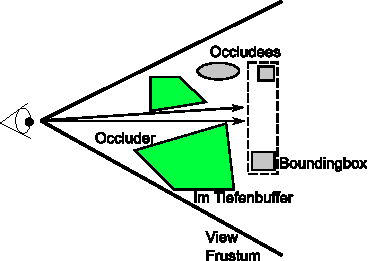
\includegraphics[scale=0.8]{images/oculling.pdf}
  \caption{Problem beim Occlusion Culling: Boundingbox zweier Objekte ist sichtbar, obwohl die darin enthaltenen Objekte verdeckt sind.}
  \label{fig:basics:oculling}
\end{figure}

\subsection{Caching}
\label{sec:basics:caching}
\todo[size=\small, inline, color=blue!40]{Kapitel: Caching}
\begin{itemize}
 \item wird über Algos gefüllt
\end{itemize}

\subsection{Speichermanagement}
\label{sec:basics:speichermanagement}
\todo[size=\small, inline, color=blue!40]{Kapitel: Speichermanagement}
\begin{itemize}
 \item nicht jeder braucht alles -> Kacheln
 \item Gewichtung über die Anzahl der Dreiecke pro Request
\end{itemize}

\section{Approximation}
\label{sec:basics:approximation}
\todo[size=\small, inline, color=blue!40]{Unterkapitel: Approximation}
Approximationen in der Computergrafik haben oft  Zurfolge, dass die Bildqualität verringert wird. Sei es weil Objekte in niedrigeren Auflösungen
\begin{itemize}
 \item Occlusion-Culling entfernt teile
 \item Nicht immer sofort ein vollständiges Bild verfügbar -> nach und nach nachladen
 \item Teile können weggelassen werden $\rightarrow$ OcclusionCulling \& FrustumCulling
 \item Begrenzung des Cache-Kontingents
 \item Tiefenbuffer Update nur alle paar Frames
 \item Sampletree
\end{itemize}
